\subsection{Verteilungssicht}
\label{sec:distribution-view}

Wie bereits im Kapitel \refsec{sec:client-server-arch} beschrieben, soll diese Anwendung als Client Server Anwendung konstruiert werden.
Dabei sind die Artefakte wie in der Abbildung \refimg{fig:client-server-deployment} strukturiert.

\begin{figure}[htb]
    \centering
    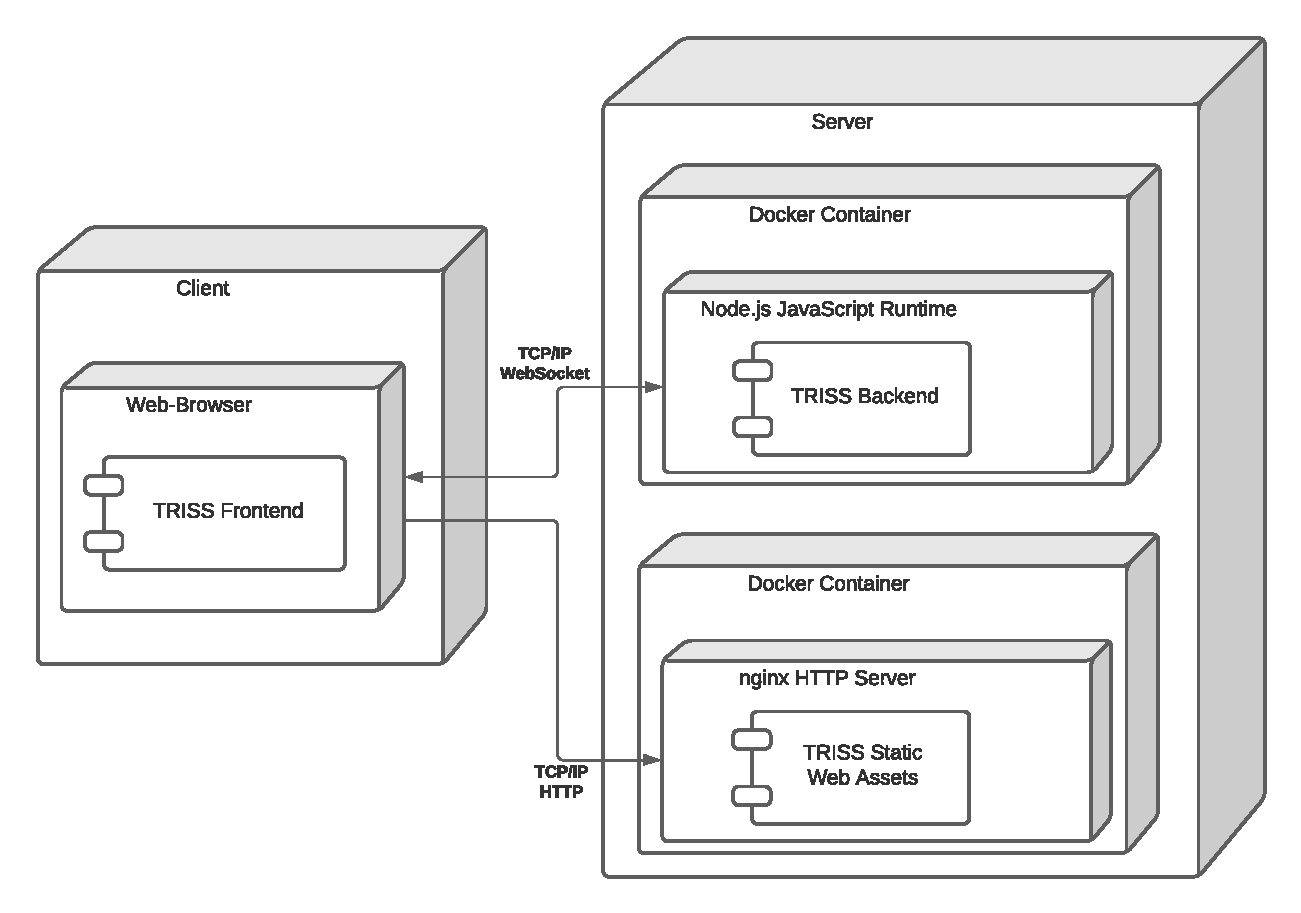
\includegraphics[scale=.65,center]{medien/abstract-client-server.pdf}
    \caption{Client Server Deployment}
    \ownsource
    \label{fig:client-server-deployment}
\end{figure}

\FloatBarrier

Die grundlegende Verteilung zieht dabei bis zu drei physische Systeme in Betracht.
Die drei Systeme würden dann jeweils eine der drei logischen Systeme bzw. deren Laufzeitumgebungen betreiben.

\newcommand{\subsubsubsection}[1]{\paragraph{#1}\mbox{}}

\subsubsection{Artefakt – TRISS Backend}

\subsubsubsection{Rolle}

Das TRISS Backend ist das zentrale System, das den Agenten betreibt sowie die Layouts und den Zustand der Welten verwaltet.

\subsubsubsection{Runtime und äußere Abhängigkeiten}

Bei diesem Artefakt handelt sich um eine JavaScript-Anwendung, die durch eine Node.js v16 Runtime betrieben wird.
Diese Runtime stellt die Standardbibliotheken wie fs, worker\_threads oder http bereit und erlaubt über npm die Verwendung weiterer Bibliotheken.

\subsubsubsection{Erzeugung}

Durch den TypeScript Compiler entsteht eine Sammlung von JavaScript-Dateien, die durch die Einstiegsdateien für den Main Thread und für den Worker eingelesen werden.
Diese werden dann in ein Image verpackt, das als Basis das \textit{node:16}\footnote{\url{https://hub.docker.com/_/node}} Image verwendet.
Als Tag\footnote{\url{https://docs.docker.com/engine/reference/commandline/tag/}} wird \textit{triss-server} genutzt.


\subsubsection{Artefakt – TRISS Frontend}

\subsubsubsection{Rolle}

Das TRISS Frontend hat die gleiche Rolle wie eine typische Webanwendung.
Sie stellt den Server-Zustand dar und erlaubt es dem Nutzer, mit diesem zu interagieren und die Welten zu inspizieren.

\subsubsubsection{Runtime und äußere Abhängigkeiten}

Sie wird durch einen modernen Webbrowser betrieben, der vor allem den Zugriff auf die notwendigen APIs bereitstellt.
So wird hier vor allem auf die OpenGL und die WebSocket API aufgebaut.

\subsubsubsection{Erzeugung}

Das Frontend wird nicht direkt erzeugt, sondern entsteht durch das Beziehen und die darauf folgende Auswertung der index.html.
Diese Komponente repräsentiert hierbei eine konkrete Instanz der Web Assets.
Das Bundle wird, wie auch alle anderen Bestandteile für das Frontend, über HTTP vom Webserver bereits gestellt.

\subsubsection{Artefakt – TRISS Static Web Assets}

\subsubsubsection{Rolle}

Die Static Web Assets repräsentieren die Ressourcen, die für den Betrieb des Frontends benötigt werden.

\subsubsubsection{Runtime und äußere Abhängigkeiten}

Dieses Artefakt wird durch einen nginx Server betrieben bzw. bereitgestellt.
Sein Betrieb benötigt keine weiteren Ressourcen.

\subsubsubsection{Erzeugung}

Gebaut werden die Assets durch Webpack.
Dieses Werkzeug generiert aus den Quelldateien sowie den referenzierten npm-Paketen ein JavaScript-Bundle und erlaubt die Auflösung der Importe innerhalb der Quelldateien.
Zusätzlich beinhalten die Web Assets neben diesem Bundle noch Medien-Dateien, CSS-Spezifikationen und die 3D-Modelle.

Nachdem Webpack dieses Bundle erzeugt hat, wird dieses, ähnlich wie bei dem TRISS Backend Artefakt, durch Docker in ein OCI Image verpackt.
Dabei dient hier das \textit{nginx:1.20}\footnote{\url{https://hub.docker.com/_/nginx}} Image als Basis.

Zusätzlich wird neben den erzeugten Dateien noch die Konfiguration mit in dem Image hinterlegt.

\subsubsection{Deployment}

Es bestehen zwei Wege, um die Anwendung in Betrieb zu nehmen.
Der erste ist, TRISS Backend und TRISS Static Web Assets einzeln aus dem Repository zu beziehen, jeweils zu bauen, die Runtimes zu konfigurieren und zu starten.

Der zweite besteht darin, die beiden Artefakte als OCI Images\footnote{\url{https://opencontainers.org/about/overview/}} zu beziehen und sie dann über eine OCI kompatible Engine zu betreiben.
Dieser zweite Weg ist der vorgesehene, da er einige Vorteile für die Entwicklung und die Inbetriebnahme mit sich bringt.

Ein zentraler Vorteil ist, dass dieses Image, ähnlich zu einer Virtual Machine, self contained ist.
Dieses Image beinhaltet alle Ressourcen, die für die Anwendung gebraucht werden.
Das beginnt bei den Betriebssystem-Schnittstellen und dessen Paketen, zusätzlichen Anwendungen, die installiert sein müssen, über die Runtime, die die Anwendung betreibt, bis hin zu den eigentlichen Dateien, die die Anwendung an sich beinhalten.

Zusätzlich sind sie für die eigentliche Entwicklung vorteilhaft, weil nur die Anforderung zu beachten ist, dass die Anwendung im Kontext eines solchen Containers laufen können muss.
Betrieben wird ein solches Image von einer OCI kompatiblen Engine, diese entkoppelt die Anwendung von dem darunterliegenden Betriebssystem und schirmt sie vollständig voneinander ab, so dass sie sich gegenseitig nicht beeinflussen können.
Somit war es nicht notwendig konkrete Betriebssystem-Versionen auszuwählen, diese zu testen und jeweils Installationsanweisungen zu formulieren.

Im Gegensatz zu einer Virtual Machine ist ein solches Image leichtgewichtiger (benötigt weniger Ressourcen und weniger Speicherplatz) und ist konkret dafür gedacht, eine einzige Anwendung zu kapseln.

Das erlaubt es auch, mit diesem Image anders umzugehen.
So kann dieses mit einem einzigen Kommando aus dem Repository bezogen und dann gestartet werden.
Der Nutzer kann dann beim Start dieses Images noch weitere Konfigurationen vornehmen, wie zum Beispiel Ports umleiten, Geräte freigeben, Hardwarenutzung limitieren, Neustart-Regeln festlegen und Partitionen persistieren.

Für diese Anwendung läuft es also dann darauf hinaus \textit{docker run\linebreak trissapp/triss-server} \textit{docker run trissapp/triss-client} auszuführen.
Näheres dazu im Kapitel \refsec{sec:artefacts}.
